\documentclass[10pt]{article}
\usepackage[T1]{fontenc}

% Document Details
\newcommand{\CLASS}{AMATH 585}
\newcommand{\assigmentnum}{Assignment 6}

\usepackage[margin = 1.15in, top = 1.25in, bottom = 1.in]{geometry}

\usepackage{titling}
\setlength{\droptitle}{-6em}   % This is your set screw
\date{}
\renewcommand{\maketitle}{
	\clearpage
	\begingroup  
	\centering
	\LARGE \sffamily\textbf{\CLASS} \Large \assigmentnum\\[.8em]
	\large Tyler Chen\\[1em]
	\endgroup
	\thispagestyle{empty}
}
 % Title Styling
\usepackage{tocloft}
\renewcommand{\cfttoctitlefont}{\Large\sffamily\bfseries}
\renewcommand{\cftsecfont}{\normalfont\sffamily\bfseries}
\renewcommand{\cftsubsecfont}{\normalfont\sffamily}
\renewcommand{\cftsubsubsecfont}{\normalfont\sffamily}

\makeatletter
\let\oldl@section\l@section
\def\l@section#1#2{\oldl@section{#1}{\sffamily\bfseries#2}}

\let\oldl@subsection\l@subsection
\def\l@subsection#1#2{\oldl@subsection{#1}{\sffamily#2}}

\let\oldl@subsubsection\l@subsubsection
\def\l@subsubsection#1#2{\oldl@subsubsection{#1}{\sffamily#2}}
 % General Styling


\usepackage{enumitem}

% Figures
\usepackage{subcaption}

% TikZ and Graphics
\usepackage{tikz, pgfplots}
\pgfplotsset{compat=1.12}
\usetikzlibrary{patterns,arrows}
\usepgfplotslibrary{fillbetween}

\usepackage{pdfpages}
\usepackage{adjustbox}

\usepackage{lscape}
\usepackage{titling}
\usepackage[]{hyperref}


% Header Styling
\usepackage{fancyhdr}
\pagestyle{fancy}
\lhead{\sffamily \CLASS}
\rhead{\sffamily Chen \textbf{\thepage}}
\cfoot{}

% Paragraph Styling
\setlength{\columnsep}{1cm}
\setlength{\parindent}{0pt}
\setlength{\parskip}{5pt}
\renewcommand{\baselinestretch}{1}

% TOC Styling
\usepackage{tocloft}
\iffalse
\renewcommand{\cftsecleader}{\cftdotfill{\cftdotsep}}

\renewcommand\cftchapafterpnum{\vskip6pt}
\renewcommand\cftsecafterpnum{\vskip10pt}
\renewcommand\cftsubsecafterpnum{\vskip6pt}

% Adjust sectional unit title fonts in ToC
\renewcommand{\cftchapfont}{\sffamily}
\renewcommand{\cftsecfont}{\bfseries\sffamily}
\renewcommand{\cftsecnumwidth}{2em}
\renewcommand{\cftsubsecfont}{\sffamily}
\renewcommand{\cfttoctitlefont}{\hfill\bfseries\sffamily\MakeUppercase}
\renewcommand{\cftaftertoctitle}{\hfill}

\renewcommand{\cftchappagefont}{\sffamily}
\renewcommand{\cftsecpagefont}{\bfseries\sffamily}
\renewcommand{\cftsubsecpagefont}{\sffamily}
\fi
 % General Styling
% Code Display Setup
\usepackage{listings,lstautogobble}
\usepackage{lipsum}
\usepackage{courier}
\usepackage{catchfilebetweentags}

\lstset{
	basicstyle=\small\ttfamily,
	breaklines=true, 
	frame = single,
	rangeprefix=,
	rangesuffix=,
	includerangemarker=false,
	autogobble = true
}


\usepackage{algorithmicx}
\usepackage{algpseudocode}

\newcommand{\To}{\textbf{to}~}
\newcommand{\DownTo}{\textbf{downto}~}
\renewcommand{\algorithmicdo}{\hspace{-.2em}\textbf{:}}
 % Code Display Setup
% AMS MATH Styling
\usepackage{amsmath, amssymb}
\newcommand{\qed}{\hfill\(\square\)}

%\newtheorem*{lemma}{Lemma} 
%\newtheorem*{theorem}{Theorem}
%\newtheorem*{definition}{Definition}
%\newtheorem*{prop}{Proposition}
%\renewenvironment{proof}{{\bfseries Proof.}}{}


% mathcal
\newcommand{\cA}{\ensuremath{\mathcal{A}}}
\newcommand{\cB}{\ensuremath{\mathcal{B}}}
\newcommand{\cC}{\ensuremath{\mathcal{C}}}
\newcommand{\cD}{\ensuremath{\mathcal{D}}}
\newcommand{\cE}{\ensuremath{\mathcal{E}}}
\newcommand{\cF}{\ensuremath{\mathcal{F}}}
\newcommand{\cG}{\ensuremath{\mathcal{G}}}
\newcommand{\cH}{\ensuremath{\mathcal{H}}}
\newcommand{\cI}{\ensuremath{\mathcal{I}}}
\newcommand{\cJ}{\ensuremath{\mathcal{J}}}
\newcommand{\cK}{\ensuremath{\mathcal{K}}}
\newcommand{\cL}{\ensuremath{\mathcal{L}}}
\newcommand{\cM}{\ensuremath{\mathcal{M}}}
\newcommand{\cN}{\ensuremath{\mathcal{N}}}
\newcommand{\cO}{\ensuremath{\mathcal{O}}}
\newcommand{\cP}{\ensuremath{\mathcal{P}}}
\newcommand{\cQ}{\ensuremath{\mathcal{Q}}}
\newcommand{\cR}{\ensuremath{\mathcal{R}}}
\newcommand{\cS}{\ensuremath{\mathcal{S}}}
\newcommand{\cT}{\ensuremath{\mathcal{T}}}
\newcommand{\cU}{\ensuremath{\mathcal{U}}}
\newcommand{\cV}{\ensuremath{\mathcal{V}}}
\newcommand{\cW}{\ensuremath{\mathcal{W}}}
\newcommand{\cX}{\ensuremath{\mathcal{X}}}
\newcommand{\cY}{\ensuremath{\mathcal{Y}}}
\newcommand{\cZ}{\ensuremath{\mathcal{Z}}}

% mathbb
\usepackage{bbm}
\newcommand{\bOne}{\ensuremath{\mathbbm{1}}}

\newcommand{\bA}{\ensuremath{\mathbb{A}}}
\newcommand{\bB}{\ensuremath{\mathbb{B}}}
\newcommand{\bC}{\ensuremath{\mathbb{C}}}
\newcommand{\bD}{\ensuremath{\mathbb{D}}}
\newcommand{\bE}{\ensuremath{\mathbb{E}}}
\newcommand{\bF}{\ensuremath{\mathbb{F}}}
\newcommand{\bG}{\ensuremath{\mathbb{G}}}
\newcommand{\bH}{\ensuremath{\mathbb{H}}}
\newcommand{\bI}{\ensuremath{\mathbb{I}}}
\newcommand{\bJ}{\ensuremath{\mathbb{J}}}
\newcommand{\bK}{\ensuremath{\mathbb{K}}}
\newcommand{\bL}{\ensuremath{\mathbb{L}}}
\newcommand{\bM}{\ensuremath{\mathbb{M}}}
\newcommand{\bN}{\ensuremath{\mathbb{N}}}
\newcommand{\bO}{\ensuremath{\mathbb{O}}}
\newcommand{\bP}{\ensuremath{\mathbb{P}}}
\newcommand{\bQ}{\ensuremath{\mathbb{Q}}}
\newcommand{\bR}{\ensuremath{\mathbb{R}}}
\newcommand{\bS}{\ensuremath{\mathbb{S}}}
\newcommand{\bT}{\ensuremath{\mathbb{T}}}
\newcommand{\bU}{\ensuremath{\mathbb{U}}}
\newcommand{\bV}{\ensuremath{\mathbb{V}}}
\newcommand{\bW}{\ensuremath{\mathbb{W}}}
\newcommand{\bX}{\ensuremath{\mathbb{X}}}
\newcommand{\bY}{\ensuremath{\mathbb{Y}}}
\newcommand{\bZ}{\ensuremath{\mathbb{Z}}}

% alternative mathbb
\newcommand{\NN}{\ensuremath{\mathbb{N}}}
\newcommand{\RR}{\ensuremath{\mathbb{R}}}
\newcommand{\CC}{\ensuremath{\mathbb{C}}}
\newcommand{\ZZ}{\ensuremath{\mathbb{Z}}}
\newcommand{\EE}{\ensuremath{\mathbb{E}}}
\newcommand{\PP}{\ensuremath{\mathbb{P}}}
\newcommand{\VV}{\ensuremath{\mathbb{V}}}
\newcommand{\cov}{\ensuremath{\text{Co}\VV}}
% Math Commands

\newcommand{\st}{~\big|~}
\newcommand{\stt}{\text{ st. }}
\newcommand{\ift}{\text{ if }}
\newcommand{\thent}{\text{ then }}
\newcommand{\owt}{\text{ otherwise }}

\newcommand{\norm}[1]{\left\lVert#1\right\rVert}
\newcommand{\snorm}[1]{\lVert#1\rVert}
\newcommand{\ip}[1]{\ensuremath{\left\langle #1 \right\rangle}}
\newcommand{\pp}[3][]{\frac{\partial^{#1}#2}{\partial #3^{#1}}}
\newcommand{\dd}[3][]{\frac{\d^{#1}#2}{\d #3^{#1}}}
\renewcommand{\d}{\ensuremath{\mathrm{d}}}

\newcommand{\indep}{\rotatebox[origin=c]{90}{$\models$}}




 % Math shortcuts
% Problem
\usepackage{floatrow}

\newenvironment{problem}[1][]
{\pagebreak
\noindent\rule{\textwidth}{1pt}\vspace{0.25em}
{\sffamily \textbf{#1}}
\par
}
{\par\vspace{-0.5em}\noindent\rule{\textwidth}{1pt}}

\newenvironment{solution}[1][]
{{\sffamily \textbf{#1}}
\par
}
{}

 % Problem Environment

\newcommand{\note}[1]{\textcolor{red}{\textbf{Note:} #1}}

\hypersetup{
   colorlinks=true,       % false: boxed links; true: colored links
   linkcolor=violet,          % color of internal links (change box color with linkbordercolor)
   citecolor=green,        % color of links to bibliography
   filecolor=magenta,      % color of file links
   urlcolor=cyan           % color of external links
}


\begin{document}
\maketitle


\begin{problem}[Problem 1]
On the course web page is a finite difference code (steady2d.m) to solve the boundary value problem:
\[
\frac{\partial}{\partial x} \left( a(x,y) \frac{\partial u}{\partial x}
\right) +
\frac{\partial}{\partial y} \left( a(x,y) \frac{\partial u}{\partial y}
\right) = f(x,y)~~~\mbox{in } (0,1) \times (0,1)
\]
\[
u(x,0) = u(x,1) = u(0,y) = u(1,y) = 0 ,
\]
where \( a(x,y) = 1 + x^2 + y^2 \) and \( f(x,y) = 1 \).
It uses a direct solver for the linear system.

Replace this direct solver first by the Jacobi method, then by the Gauss Seidel method, and then by the SOR method. For each method, make a plot of the relative residual norm, \( \| b - A u^k \| / \| b \| \) versus iteration number \( k \). (Use a logarithmic scale for the residual; i.e., you may use \verb+semilogy+
in Matlab to do the plot.) Try several different values for the parameter \( \omega \) in SOR, until you find one that seems to work well.

Then try solving the linear system using the conjugate gradient method.  You may write your own CG code or use the one in Matlab (called {\bf pcg}).  First try CG without a preconditioner (i.e., with preconditioner equal to the identity) and then try CG with the Incomplete Cholesky decomposition as the preconditioner. You may use \verb+ichol+ in Matlab to generate the incomplete Cholesky decomposition.  Again make a plot of relative residual norm versus iteration number for the CG method.

Experiment with a few different mesh sizes and comment on how the number of iterations required to reach a fixed level of accuracy seems to vary with \( h \) for each method.
\end{problem}

\begin{solution}[Solution]

We implement Jacobi iteration, Gauss-Seidel, and successive over relaxation:
\lstinputlisting[linerange=\#<startJacobi>-\#<endJacobi>]{hw6_1.py}
\lstinputlisting[linerange=\#<startGS>-\#<endGS>]{hw6_1.py}
\lstinputlisting[linerange=\#<startSOR>-\#<endSOR>]{hw6_1.py}

Note that we use a incomplete LU decomposition to compute a preconditioner for the conjugate gradient method. This is done using Scipy's sparse package as:
\lstinputlisting[linerange=\#<startCG>-\#<endCG>]{hw6_1.py}

Figure~\ref{convergence} shows how the residual of each of these methods vs the iteration number. As expected Gauss-Seidel converges about twice as fast as Jacobi. Successive over relaxation converges faster than either of these methods, with the rate depending on the choice of \( \omega \).
\begin{figure}[H]\centering
    \begin{subfigure}{.6\textwidth}
        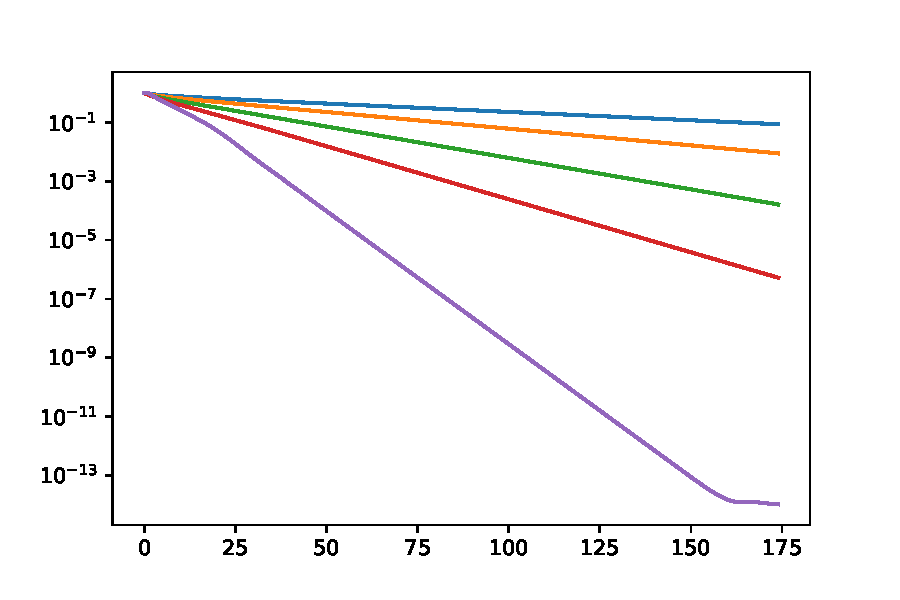
\includegraphics[width=\textwidth]{img/1/iter_convergence_20.pdf}
    \end{subfigure}
    \begin{subfigure}{.25\textwidth} \small
        blue: Jacobi\\
        orange: GS \\
        green: SOR (\( \omega = 1.3 \)) \\
        red: SOR (\( \omega = 1.5 \)) \\
        purple: SOR (\( \omega = 1.7 \))
    \end{subfigure}
\caption{Residual norm vs. iteration count with \( n=20 \) for simple iterative methods}
\end{figure}
\begin{figure}[H]\centering
    \begin{subfigure}{.6\textwidth}
        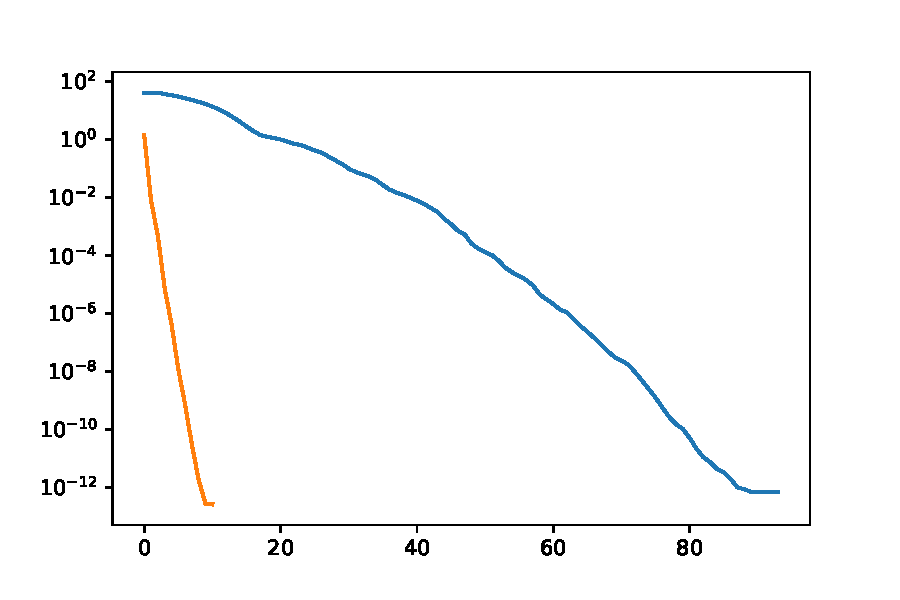
\includegraphics[width=\textwidth]{img/1/cg_convergence_20.pdf}
    \end{subfigure}
    \begin{subfigure}{.25\textwidth}
        blue: no preconditioner \\
        orange: iLU preconditioner
    \end{subfigure}
\caption{Residual norm vs. iteration count with \( n=20 \) for conjugate gradient methods}
\label{convergence}
\end{figure}

Figures~\ref{itervsh} and \ref{itervshcg} show the number of iterations required to reach the specified tolerance for Jacobi iteration, Gauss-Seidel iteration, successive over relaxation at varying \( \omega \), conjugate gradient, and conjugate gradient using the preconditioner described above. All methods take longer to converge as the size of the system increases. However, using a preconditioner means that the number of iterations does not increase significantly.

Jacobi and Gauss-Seidel iteration require significantly more iterations as the system size increases. Successive over relaxation does seems to remain relatively constant until some threshold size at which point the number of iterations begins to increase rapidly. This may be explained by the choice of \( \omega \). We expect that as the system size increases that the optimal value of omega converges to 2. As seen in the figure, the higher values of \( \omega \) worked fine for longer.

\begin{figure}[H]\centering
    \begin{subfigure}{.6\textwidth}
        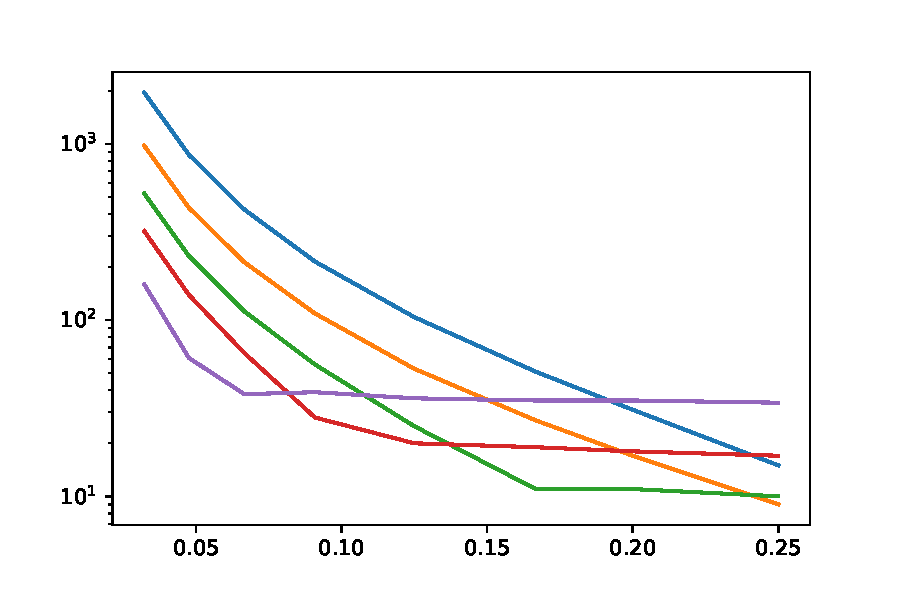
\includegraphics[width=\textwidth]{img/1/iter_vs_h.pdf}
    \end{subfigure}
    \begin{subfigure}{.25\textwidth}
        blue: Jacobi\\
        orange: GS \\
        green: SOR (\( \omega = 1.3 \)) \\
        red: SOR (\( \omega = 1.5 \)) \\
        purple: SOR (\( \omega = 1.7 \))
    \end{subfigure}
\iffalse
    \begin{subfigure}{.6\textwidth}
        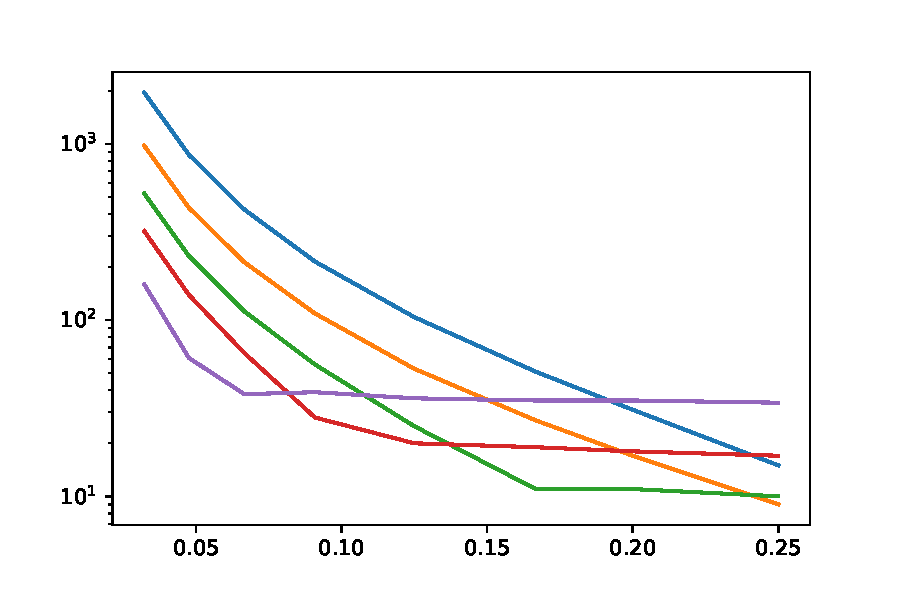
\includegraphics[width=\textwidth]{img/1/iter_vs_h.pdf}
    \end{subfigure}
    \begin{subfigure}{.25\textwidth}
        \hspace{1em}
   \end{subfigure}
\fi
    \caption{Iterations needed (log scale) to reach tolerance of \( 10^{-5} \) vs. mesh size.}% (both figures are of the same data with different horizontal scales)}
    \label{itervsh}
\end{figure}

\begin{figure}[H]\centering
    \begin{subfigure}{.6\textwidth}
        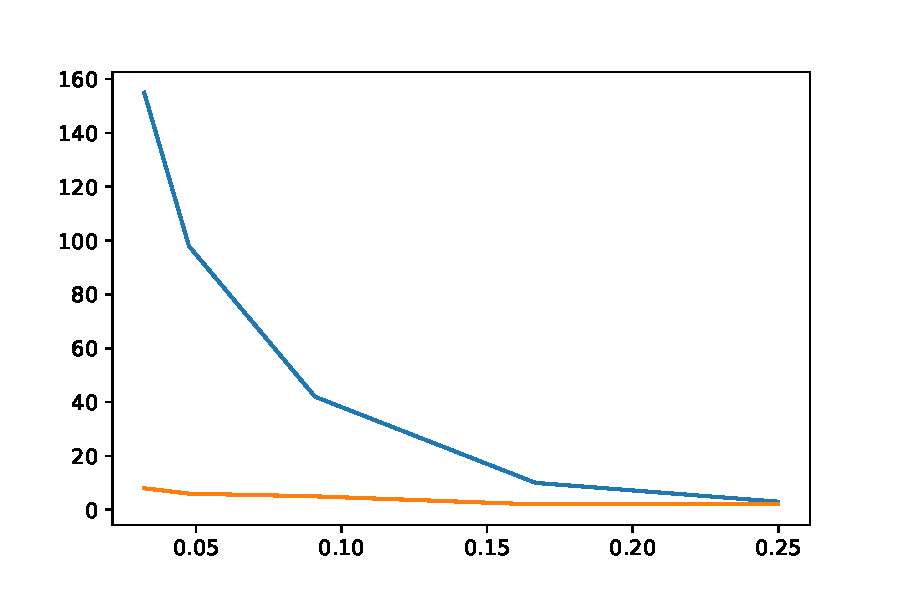
\includegraphics[width=\textwidth]{img/1/iter_vs_h_cg.pdf}
    \end{subfigure}
    \begin{subfigure}{.25\textwidth}
        blue: no preconditioner \\
        orange: iLU preconditioner
    \end{subfigure}
    \caption{Iterations to reach tolerance of \( 10^{-16} \) vs. mesh size}
    \label{itervshcg}
\end{figure}

\end{solution}

\begin{problem}[Problem 2]
Suppose a symmetric positive definite matrix \( A \) has one thousand eigenvalues uniformly distributed between \( 1 \) and \( 10 \), and one eigenvalue of \( 10^4 \). Suppose another symmetric positive definite matrix \( B \) has an eigenvalue of \( 1 \) and has one thousand eigenvalues uniformly distributed between \( 10^3 \) and \( 10^4 \). Since each matrix has condition number \( \kappa = 10^4 \), we have seen that the error at step \( k \) of the CG algorithm satisfies
    \[
\frac{\| e^{(k)} \|_{A,B}}{\| e^{(0)} \|_{A,B}} \leq 2 \left( \frac{
\sqrt{\kappa} - 1}{\sqrt{\kappa} +1} \right)^k = 2 \left( \frac{99}{101} 
\right)^k .
\]
Give another bound on \( \| e^{(k)} \|_A / \| e^{(0)} \|_A \) based on a polynomial that is a product of a degree \( k-1 \) Tchebyshev polynomial on the interval \( [1,10] \) and a linear polynomial that is \( 1 \) at the origin and \( 0 \) at \( 10^4 \).  Give another bound on \( \| e^{(k)} \|_B / \| e^{(0)} \|_B \)  based on a polynomial that is a product of a degree  \( k-1 \) Tchebyshev polynomial on the interval \( [ 10^3 , 10^4] \) and a linear polynomial that is \( 1 \) at the origin and \( 0 \) at \( 1 \).  For which matrix would you expect CG to converge more rapidly?  [If you are not sure, you may try it in Matlab.]
\end{problem}

\begin{solution}[Solution]

Let \( P_k(x) \) be the polynomial constructed implicitly by the conjugate gradient method for a (reasonable) matrix \( X \). That is, 
\begin{align*}
    P_k = \operatorname{argmin}_{P\in \mathcal{P} _k} \norm{P(A)e_0}_X
\end{align*}

Recall that for any polynomial, \( P(x) \) we have,
\begin{align*}
    \dfrac{\norm{e^{(k)}}_X}{\norm{e^{(0)}}_X}  
    = \dfrac{\norm{P_k(A)e_0}_X}{\norm{e_0}_X} 
    \leq \dfrac{\norm{P(A)e_0}_X}{\norm{e_0}_X} 
    \leq \max_{1\leq j\leq m} |P(\lambda_j)|    
\end{align*}

Recall further that,
\begin{align*}
    \left|  \frac{T_{k}(1)}{T_{k} \left( \frac{\lambda_{b}+\lambda_a}{\lambda_{b} - \lambda_a} \right)}  \right| \leq 2 \left( \dfrac{\sqrt{\kappa'}-1}{\sqrt{\kappa'}+1} \right)^{k-1}, && \kappa' = \dfrac{\lambda_{b}}{\lambda_a}
\end{align*}

Let \( \{\lambda_j\}_{j=1}^{m} \) be the eigenvalues of \( A \) in order. That is \( \lambda_1 = 1, \lambda_{m-1} = 10, \lambda_m = 10^4 \).
Define,
\begin{align*}
    \tilde{P}_{A,k}(x) = \dfrac{T_{k-1} \left( \frac{\lambda_{m-1}+\lambda_1-2x}{\lambda_{m-1}-\lambda_1} \right)}{T_{k-1} \left( \frac{\lambda_{m-1}+\lambda_1}{\lambda_{m-1} - \lambda_1} \right)} \left( \dfrac{\lambda_m-x}{\lambda_m} \right)
\end{align*}

Clearly \( \tilde{P}_{A,k}(\lambda_m) = 0 \). We therefore know \( \max_{j}\tilde{P}_{A,k}(\lambda_j) \) is attained for some \( \lambda_j \in \), \( j=1,\ldots, m-1 \). Since \( T_k \) attains its maximum on \( [0,1] \) at the boundaries, and since \( |\lambda_m-x| \) is strictly decreasing on \( [\lambda_1,\lambda_{m-1}] \), we know,
\begin{align*}
    \max_j |\tilde{P}_{A,k} (\lambda_j) | = | \tilde{P}_{A,k} (\lambda_{1}) | 
\end{align*}

Thus, with \( \kappa_A = \lambda_{m-1} / \lambda_1 = 10 \) and \( |\lambda_m-\lambda_1|/|\lambda_m| = (10^4-1)/10^4 \leq 1 \),
\begin{align*}
    \dfrac{\norm{e^{(k)}}_A}{\norm{e^{(0)}}_A} 
    %\leq \dfrac{T_{k-1}(1)}{T_{k-1} \left( \frac{\lambda_{m-1} + \lambda_1}{\lambda_{m-1}-\lambda_1} \right)}\left( \dfrac{\lambda_m - \lambda_{m-1}}{\lambda_m} \right) 
    \leq 2 \left( \dfrac{\sqrt{\kappa_A}-1}{\sqrt{\kappa_A}+1} \right)^{k-1} \left| \dfrac{\lambda_m-\lambda_{1}}{\lambda_m} \right|
    \leq 2 \left( \dfrac{\sqrt{10}-1}{\sqrt{10}+1} \right)^{k-1}
\end{align*}

Now, let \( \{\gamma_j\}_{j=1}^{m} \) be the eigenvalues of \( B \) in order. That is \( \gamma_1 = 1, \gamma_{2} = 10^3, \gamma_m = 10^4 \).
Define,
\begin{align*}
    \tilde{P}_{B,k}(x) = \dfrac{T_{k-1} \left( \frac{\gamma_{m-1}+\gamma_1-2x}{\gamma_{m-1}-\gamma_1} \right)}{T_{k-1} \left( \frac{\gamma_{m-1}+\gamma_1}{\gamma_{m-1} - \gamma_1} \right)} \left( \dfrac{\gamma_1-x}{\gamma_1} \right)
\end{align*}

Clearly \( \tilde{P}_{A,k}(\gamma_1) = 0 \). We therefore know \( \max_{j}\tilde{P}_{A,k}(\gamma_j) \) is attained for some \( \gamma_j \in \), \( j=1,\ldots, m-1 \). Since \( T_k \) attains its maximum on \( [0,1] \) at the boundaries, and since \( |\gamma_1-x| \) is strictly increasing on \( [\gamma_2,\gamma_m] \), we know,
\begin{align*}
    \max_j |\tilde{P}_{A,k} (\gamma_j) | = | \tilde{P}_{A,k} (\gamma_{m}) | 
\end{align*}

Thus, with \( \kappa_B = \gamma_{m} / \gamma_2 = 10 \) and \( |\gamma_1-\gamma_m|/|\gamma_1| = (10^4-1)/1 \leq 10^4 \),
\begin{align*}
    \dfrac{\norm{e^{(k)}}_B}{\norm{e^{(0)}}_B} 
    %\leq \dfrac{T_{k-1}(1)}{T_{k-1} \left( \frac{\gamma_{m-1} + \gamma_1}{\gamma_{m-1}-\gamma_1} \right)}\left( \dfrac{\gamma_m - \gamma_{m-1}}{\gamma_m} \right) 
    \leq 2 \left( \dfrac{\sqrt{\kappa_B}-1}{\sqrt{\kappa_B}+1} \right)^{k-1} \left| \dfrac{\gamma_1-\gamma_{m}}{\gamma_1} \right|
    \leq 20000 \left( \dfrac{\sqrt{10}-1}{\sqrt{10}+1} \right)^{k-1}
\end{align*}

Presumably conjugate gradient applied to \( A \) will converge faster as the bound on convergence is much better. However we have not proved this here as our bounds are only upper bounds.


\end{solution}

\begin{problem}[Problem 3]
Repeat the experiments on p.~103 of the text, leading to Figures 4.8 and4.9, but use the Gauss-Seidel method and (unpreconditioned) CG instead of Jacobi iteration.  That is, set up difference equations for the problem
\[
u''(x) = f(x),~~~u(0) = 1 ,~u(1) = 3 ,
\]
where
\[
f(x) = -20 + a \phi'' (x) \cos( \phi (x)) - a ( \phi' (x) )^2 \sin ( \phi (x) ),
\]
where \( a = 0.5 \) and \( \phi (x) = 20 \pi x^3 \).  The true solution is
\[
u(x) = 1 + 12 x - 10 x^2 + a \sin ( \phi (x) ) .
\]
Starting with initial guess \( u^{(0)} \) with components \( 1 + 2 x_i \), \( i=1, \ldots , 255 \), run, say, \( 20 \) Gauss-Seidel iterations and then
\( 20 \) CG iterations, plotting the true solution to the linear system and the approximate solution, say, at steps 0, 5, 10, and 20, and 
also plotting the error (the difference between true and approximate solution).  Print the size of the error (the \( L_2 \)-norm or the \( \infty \)-norm) at these steps too.  Based on your results, would you say that Gauss-Seidel and CG would be effective smoothers for a multigrid method?
\end{problem}

\begin{solution}[Solution]

We would like to solve \( Au = b \) where, \( A \) has \( -2/h^2 \) on the main diagonal and \( 1/h^2 \) on the off diagonals, and \( b \) is \( f \) evaluated on the grid where we subtract \( 1/h^2 \) from the first entry of \( b \) and \( 3/h^2 \) from the last entry to take care of the boundary conditions.

To ensure \( A \) is positive definite we multiply both sides by \( -1 \).

Figures~\ref{gs} and \ref{cg} show the approximate solution (orange) and the actual solution (blue) on the top figures. The bottom figure is the difference of the two. 

Both seem like they would work fine as smoothers for multigrid methods as high frequency parts of the error are reduced quickly.

\begin{figure}[H]\centering
    \foreach \k in {0,5,10,20}{
        \begin{subfigure}{.23\textwidth}\centering
            \includegraphics[width=\textwidth]{img/3/GS_sol_\k.pdf}
            \includegraphics[width=\textwidth]{img/3/GS_diff_\k.pdf}
            \( \norm{\text{error}}_{L_2} =  \) \input{img/3/GS_err_\k.txt}
            \caption{\( k = \k \)}
        \end{subfigure}        
    }
\caption{Gauss Seidel Method}
\label{gs}
\end{figure}

    \begin{figure}[H]\centering
    \foreach \k in {0,5,10,20}{
        \begin{subfigure}{.23\textwidth}\centering
            \includegraphics[width=\textwidth]{img/3/cg_sol_\k.pdf}
            \includegraphics[width=\textwidth]{img/3/cg_diff_\k.pdf}
            \( \norm{\text{error}}_{L_2} =  \) \input{img/3/cg_err_\k.txt}
            \caption{\( k = \k \)}
        \end{subfigure}        
    }
\caption{Conjugate Gradient Method}
\label{cg}
\end{figure}

\end{solution}

\end{document}
